% Performance Comparison Figure Reference
% This figure shows the analysis of different inference strategies
% comparing Context Ensemble, Image-Level Retrieve, Object-Level Retrieve, and In-Context Tuning
% across different percentages of context samples used (1% to 100%)
% 
% Figure dimensions: Standard CVPR figure width
% Figure type: Line plot with multiple series
% X-axis: Percentage of Context Sample Used (%)
% Y-axis: OOD Dice (%)
% Series: 4 different inference strategies
%
% To include this figure in LaTeX:
% \begin{figure}[t]
%   \centering
%   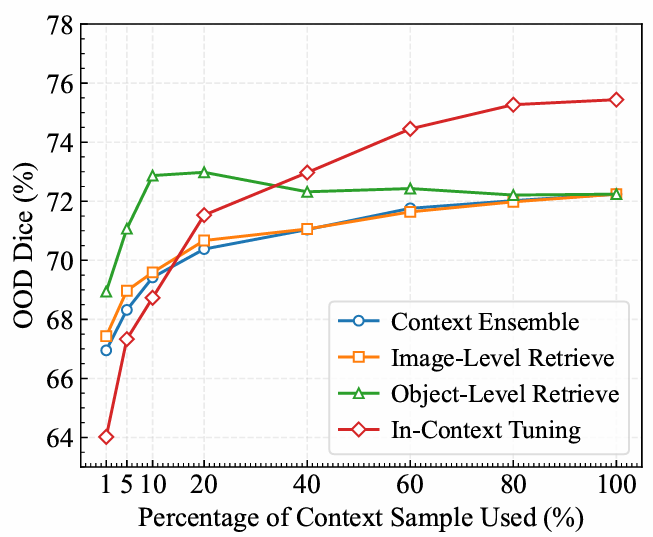
\includegraphics[width=0.8\linewidth]{fig/performance_comparison.png}
%   \caption{Analysis of different inference strategies showing out-of-distribution performance across varying percentages of context samples. In-Context Tuning demonstrates superior performance scaling, reaching approximately 75.5\% Dice score, while other methods plateau around 72\% Dice score.}
%   \label{fig:performance_comparison}
% \end{figure}
